\documentclass{article}

% If accepted, swap to package below for authorship listing
% \usepackage{icml2026}
\usepackage[accepted]{icml2026}

% Additional packages
\usepackage{amsmath,amssymb,amsthm}
\usepackage{graphicx}
\usepackage{booktabs}
\usepackage{hyperref}
\usepackage{url}
\usepackage{xcolor}
\usepackage{microtype}
\usepackage{algorithm}
\usepackage{algpseudocode}
\usepackage{bm}
\captionsetup{labelfont=bf, textfont=normalfont}

% Double-blind submission
\icmltitlerunning{Graph Learning on Ensembles of Cyclic Peptides}

\begin{document}

\twocolumn[
\icmltitle{%
  Graph Learning on Ensembles of Cyclic Peptides:\\
  An Investigation of Molecular Ensemble Modeling
}

\begin{icmlauthorlist}
    \icmlauthor{Aaron Feller}{ut,novo}
    \icmlauthor{Maxim Secor}{novo}
    \icmlauthor{Kris Deibler}{novo}
\end{icmlauthorlist}

\icmlaffiliation{ut}{Interdisciplinary Life Sciences, University of Texas at Austin, Austin, TX.}
\icmlaffiliation{novo}{Molecular AI, Novo Nordisk, Lexington, MA}

\icmlcorrespondingauthor{Aaron Feller}{aaron.feller@utexas.edu}

\icmlkeywords{%
  graph neural networks,
  peptide conformation,
  molecular graph foundation models,
  conformer ensembles,
  inverse folding,
  geometric deep learning
}

\vskip 0.3in
]

\printAffiliationsAndNotice{}

% ============================================================
\begin{abstract}
% ============================================================
Molecular property prediction from structure often uses a single representative conformation, even though many molecules exist as conformational ensembles in solution. We introduce \textbf{EnsembleEGNN}, a molecular ensemble foundation model that encodes an ensemble by first encoding each conformer with shared Equivariant Graph Neural Network (EGNN) layers, then pooling the resulting conformer representations with a Set Attention Block. We pretrain the model on CREMP, a cyclic peptide ensemble dataset, using a multi-task self-supervised objective combining masked token recovery, noisy-coordinate reconstruction, and pairwise distance reconstruction. On the CREMP-CycPeptMPDB dataset, training EnsembleEGNN from scratch fails entirely ($R^2=0.005$). However, the pretrained model reaches $R^2=0.477$ and Pearson $r=0.699$, outperforming the sequence-only BERT baseline ($R^2=0.439$, Pearson $r=0.667$). When EnsembleEGNN is co-trained end-to-end with the BERT sequence encoder, the hybrid model improves further to $R^2=0.538$ and Pearson $r=0.737$. These results demonstrate that encoding conformational ensembles into a single thermodynamically informed embedding improves cyclic-peptide property prediction.
\end{abstract}

% ============================================================
\section{Introduction}
\label{sec:intro}
% ============================================================

Graph foundation models (GFMs) aim to pretrain once and transfer across node, edge, and graph-level tasks with minimal fine-tuning~\citep{liu2025graph}. In the molecular domain, GFMs have shown promise for small molecules and proteins~\citep{mendez2024mole, hsu2022learning}, yet a fundamental representational mismatch persists. In solution, many molecules do not occupy a single static structure but are understood as Boltzmann-weighted ensembles of conformers~\citep{chandler1987introduction, tuckerman2023statistical}. This mismatch is particularly detrimental for cyclic peptides \cite{hui2025molecular, bayaraa2026fast, damjanovic2021elucidating}. These scaffolds are inherently flexible, and their thermodynamic ensembles ultimately dictate critical properties like membrane permeability, protease resistance, and target binding~\citep{yudin2015macrocycles, calvo2025computational}.

\paragraph{The conformer aggregation problem.}
Structure-based methods typically process single conformers~\citep{otero2025pepmnet, liu2026molx} or apply naive pooling~\citep{zhu2024learning}. For flexible cyclic peptides, this discards critical thermodynamic context regarding how atoms move across accessible states. The core challenge remains: given $C$ conformers of $N$ atoms with Boltzmann weights $(w_c)$, how can a model efficiently aggregate this geometric information into a single embedding? With conformer-generation pipelines improving~\citep{aranganathan2025modeling}, models that can encode at the ensemble level will become increasingly useful.

\paragraph{Our approach.}
EnsembleEGNN encodes each conformer separately with a shared equivariant graph neural network (EGNN) \cite{satorras2021en} and then combines those conformer-level representations into a single ensemble embedding. In this view, the same ordered set of atoms is observed under multiple 3D conformations, allowing the model to explicitly capture the inherent flexibility of the molecule. By pretraining on Boltzmann-weighted atom embeddings across $C$ conformer states, the model is forced to aggregate geometric context across the ensemble (Figure~\ref{fig:hypergraph_concept}). The conformers are then pooled using a set attention block \cite{lee2019set}, allowing for the attention mechanism to learn prioritization of conformers that are important on a per-task basis. This design maintains low complexity while still learning from the full thermodynamic distribution rather than from a single static structure.

\paragraph{Contributions.}
We present three main contributions: \textbf{(1)} an ensemble geometric encoder that learns a single embedding from multiple conformers using set attention pooling; \textbf{(2)} a multi-task pretraining objective with masked token recovery, noisy-coordinate reconstruction, and distance reconstruction that leverages Boltzmann-informed atom pooling, evaluated with CREMP~\citep{grambow2024cremp}; and \textbf{(3)} cross-validation on CREMP-CycPeptMPDB to predict membrane permeability, demonstrating that a) pretraining is necessary and b) conformer-aware geometric modeling improves over a sequence-encoder baseline.

\begin{figure*}[t]
  \centering
  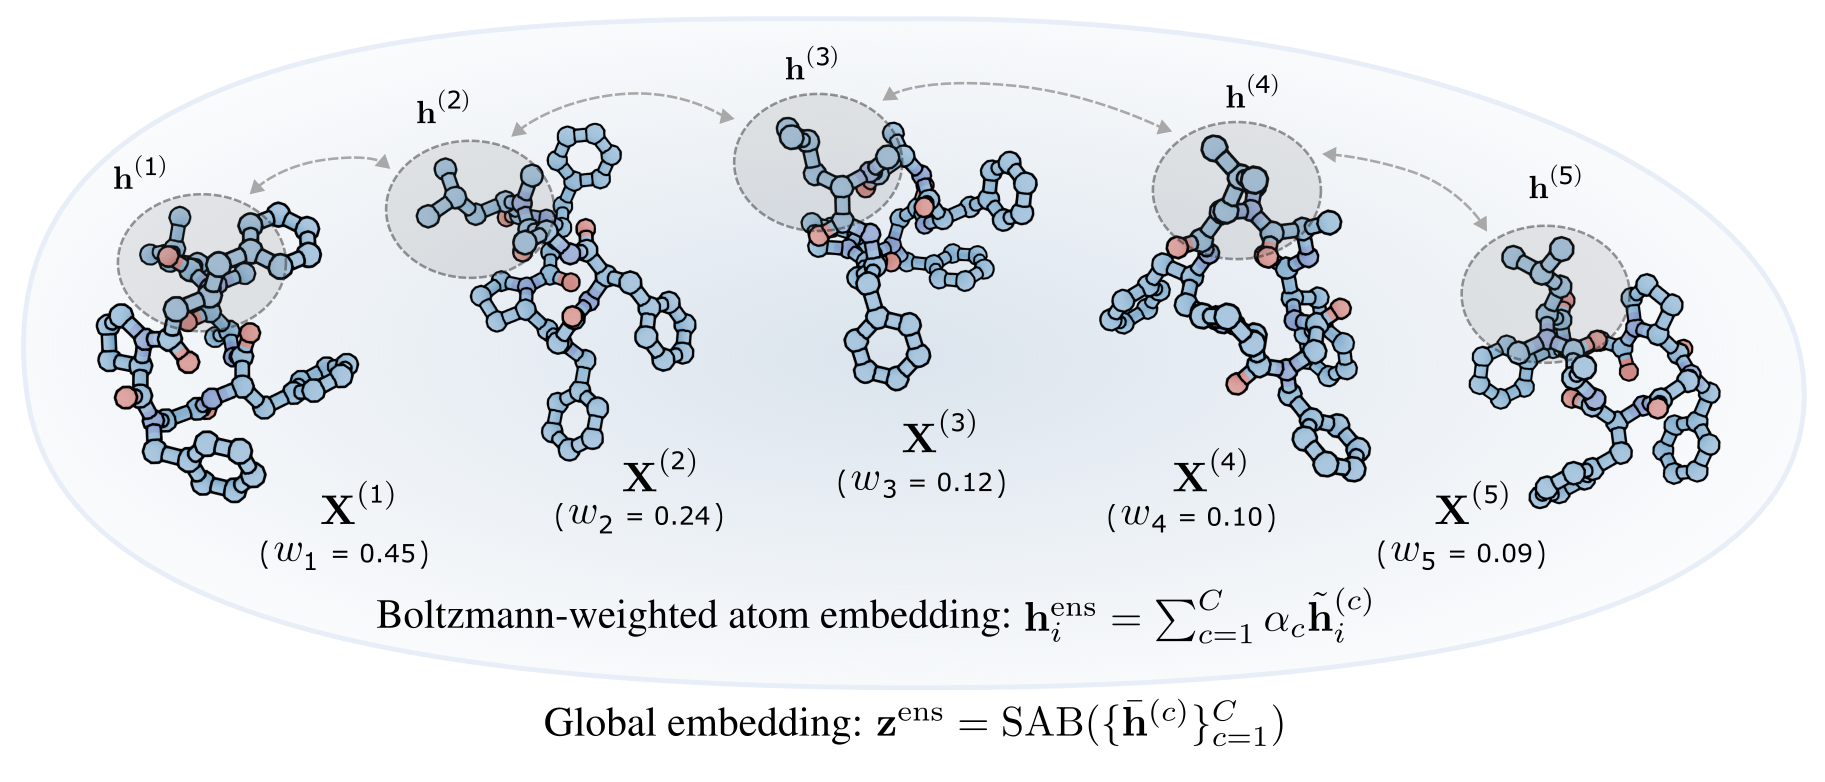
\includegraphics[width=0.8\textwidth]{figures/graphical_abstract.png}
  \caption{\textbf{Information flow and conformer aggregation in EnsembleEGNN.} The model processes a thermodynamic ensemble of $C$ distinct spatial states, each defined by 3D coordinates $\mathbf{X}^{(c)}$ and a Boltzmann weight $w_c$. The shaded regions highlight the local $k$-nearest-neighbor graph of a single shared atom (node $i$) across the ensemble. After per-conformer EGNN layers update the local geometry, the finalized node features ($\tilde{\mathbf{h}}_i^{(c)}$) are aggregated via a Boltzmann-informed attention mechanism ($\alpha_c$) to produce a single unified atom embedding ($\mathbf{h}_i^{\text{ens}}$). Finally, a Set Attention Block (SAB) reasons over the entire collection of conformers to generate a macroscopic global embedding ($\mathbf{z}^{\text{ens}}$) for downstream property prediction.}
  \label{fig:hypergraph_concept}
\end{figure*}

% ============================================================
\section{Method}
\label{sec:method}
% ============================================================

\subsection{Data Representation for Conformer Ensembles}
\label{sec:data-representation}

To bridge 1D token identity and 3D geometry, we represent each peptide as a set of atom tokens, with multiple conformations that reuse the same nodes with different position coordinates.

Each molecule contains three pieces of information: node (atom) identities ($a$), 3D conformer coordinates ($X$), and conformer weights ($w$). In the all-atom experiments used in this paper, the node tokens are atom-level tokens and the coordinates are all-atom conformer coordinates. The goal of the model is to a) formulate pretraining tasks for ensembles, and b) compress an ensemble into a single embedding that can be used for downstream prediction.

To construct these inputs from CREMP~\citep{grambow2024cremp}, we extract all available conformers, rank them by their Boltzmann weights, retain the top $C=5$ states, and renormalize those weights to sum to one before serialization. Node (atom) tokens ($a$) correspond directly to atom identities, giving a coordinate tensor of shape $C \times a \times 3$ together with per-conformer weights.

\subsection{Architecture}
\label{sec:arch}

\paragraph{Conformer-wise encoding.}
Each conformer is processed through $L$ EGNN layers~\citep{satorras2021en}. The model updates both the node features and coordinates by passing messages exclusively over the local $k$-nearest-neighbor graph within that specific conformer, shown here:

\begin{equation}
  \mathbf{h}_i^{(c,\ell+1)}, \mathbf{x}_i^{(c,\ell+1)}
  = \mathrm{EGNNLayer}\!\left(
      \mathbf{h}_i^{(c,\ell)},\,
      \mathbf{x}_i^{(c,\ell)},\,
      \mathcal{N}_k(i, c)
    \right)
\end{equation}

where the initial node features are $\mathbf{h}_i^{(c,0)} = \mathrm{Embed}(a_i)$, the initial coordinates are $\mathbf{x}_i^{(c,0)} = \mathbf{X}_i^{(c)}$, and $\mathcal{N}_k(i,c)$ denotes the $k$ nearest spatial neighbors of node $i$ in conformer $c$. This restriction to a specified set of neighbors allows for the model to extend to any molecule size and enables straightforward pretraining.

The choice of EGNN layers ensures that the per-conformer message passing is strictly equivariant to rotations and translations in 3D space. This property allows the model to learn robust geometric representations without relying on expensive coordinate frame alignments or spatial data augmentation.

\paragraph{Conformer fusion.}
Let $\tilde{\mathbf{h}}^{(c)} \in \mathbb{R}^{N \times d}$ denote the final post-EGNN node (i.e. atom) features for conformer $c$. To pool these separate structures into a unified representation, each conformer receives an attention weight driven by two signals: a learned score from the mean ensemble embedding and a thermodynamic prior from the Boltzmann weight. We compute these attention weights as:

\begin{equation}
  \alpha_c = \frac{\exp\!\left(f_\phi(\bar{\mathbf{h}}^{(c)}) + \log w_c\right)}
  {\sum_{c'}\exp\!\left(f_\phi(\bar{\mathbf{h}}^{(c')}) + \log w_{c'}\right)}
\end{equation}

where $\bar{\mathbf{h}}^{(c)} = \frac{1}{N}\sum_i \tilde{\mathbf{h}}_i^{(c)}$ is the mean node feature for conformer $c$ and $f_\phi$ is a 2-layer MLP. 

Using these attention weights, we compute two distinct ensemble embeddings:

\begin{equation}
  \mathbf{h}_i^{\mathrm{ens}} = \sum_{c=1}^C \alpha_c\,\tilde{\mathbf{h}}_i^{(c)},
  \qquad
  \mathbf{z}^{\mathrm{ens}} = \mathrm{SAB}\!\left(\{\bar{\mathbf{h}}^{(c)}\}_c\right)
\end{equation}

The first term, $\mathbf{h}_i^{\mathrm{ens}}$, is a per-atom embedding obtained by taking the attention-weighted average of each atom across all conformers. The second term, $\mathbf{z}^{\mathrm{ens}} \in \mathbb{R}^d$, is a global graph-level embedding generated by passing the conformer embeddings through a Set Attention Block (SAB)~\citep{lee2019set}. 

Utilizing SAB with inducing points reduces the conformer fusion complexity from $O(N^2)$ with quadratic attention to $O(nm)$, enabling efficient scaling across large conformational ensembles.

\begin{algorithm}[h]
   \caption{EnsembleEGNN Conformer-Aware Fusion Forward Pass}
   \label{alg:fusion}
\begin{algorithmic}[1]
   \State {\bfseries Input:} Peptide with $N$ atoms having: 
   \Statex \hspace{1.1cm} atom types $\{a_i\}_{i=1}^N$,
   \Statex \hspace{1.1cm} per-conformer atom coordinates $\{\mathbf{X}^{(c)}\}_{c=1}^C$, 
   \Statex \hspace{1.1cm} and Boltzmann weights $\{w_c\}_{c=1}^C$
   \State Initialize atom features $\mathbf{h}_i^{(c,0)} = \mathrm{Embed}(a_i)$
   \For{$\ell = 0$ {\bfseries to} $L-1$}
       \State Update $\mathbf{h}_i^{(c,\ell+1)}, \mathbf{x}_i^{(c,\ell+1)}$ via EGNN 
   \EndFor
   \State Let $\tilde{\mathbf{h}}^{(c)} = \mathbf{h}^{(c,L)}$ denote final atom features
   \For{$c = 1$ {\bfseries to} $C$}
       \State Conformer token: $\bar{\mathbf{h}}^{(c)} = \frac{1}{N} \sum_{i=1}^N \tilde{\mathbf{h}}_i^{(c)}$
       \State Attention logit: $u_c = f_\phi(\bar{\mathbf{h}}^{(c)}) + \log w_c$
   \EndFor
   \State Attention weights: $\alpha_c = \frac{\exp(u_c)}{\sum_{c'} \exp(u_{c'})}$
   \State Ensemble atoms: $\mathbf{h}_i^{\mathrm{ens}} = \sum_{c=1}^C \alpha_c \tilde{\mathbf{h}}_i^{(c)}$
   \State Global embedding: $\mathbf{z}^{\mathrm{ens}} = \mathrm{SAB}(\{\bar{\mathbf{h}}^{(c)}\}_{c=1}^C)$
   \State {\bfseries Output:} $\mathbf{h}^{\mathrm{ens}}$ and $\mathbf{z}^{\mathrm{ens}}$
\end{algorithmic}
\end{algorithm}

% \paragraph{Task heads.}
% The shared backbone supports three pretraining objectives and one downstream fine-tuning head. For pretraining, we apply a linear classifier to the Boltzmann weighted per-atom embeddings $\mathbf{h}_i^{\mathrm{ens}}$ for masked token recovery, we compare the EGNN-refined conformer coordinates directly against the original clean coordinates for noisy-coordinate reconstruction, and we apply a pairwise L1 loss to projected per-atom embeddings for distance reconstruction. For downstream property regression, we fine-tune a 2-layer MLP on the global ensemble embedding $\mathbf{z}^{\mathrm{ens}}$.

\subsection{pretraining Objective}
\label{sec:pretrain}

During pretraining, we corrupt both the node identities and the coordinates. We randomly select 15\% of valid node positions for masked-token supervision. Following a BERT-style corruption scheme, 80\% of those selected positions are replaced with a mask token, 10\% are replaced with a random token, and 10\% are left unchanged. 

We also add Gaussian noise to valid node and conformer positions, producing a noisy coordinate tensor that the model must refine back toward the clean structure.

The composite pretraining loss is:

% \begin{equation}
%   \mathcal{L} = \lambda_{\mathrm{tok}} \mathcal{L}_{\mathrm{tok}}
%               + \lambda_{\mathrm{coord}} \mathcal{L}_{\mathrm{coord}}
%               + \lambda_{\mathrm{dist}} \mathcal{L}_{\mathrm{dist}}
% \end{equation}

\begin{equation}
  \mathcal{L} = 0.3 (\mathcal{L}_{\mathrm{tok}})
              + 0.5 (\mathcal{L}_{\mathrm{coord}})
              + 0.2 (\mathcal{L}_{\mathrm{dist}})
\end{equation}


The masked-token term $(\mathcal{L}_{\mathrm{tok}})$ is a cross-entropy loss computed at the masked valid nodes, training the per-atom embeddings to recover the original token identities from corrupted inputs. The coordinate term $(\mathcal{L}_{\mathrm{coord}})$ is an MSE loss between the final EGNN-refined coordinates and the clean conformer coordinates, training the geometric backbone to denoise each conformer. 

The distance term $(\mathcal{L}_{\mathrm{dist}})$ compares pairwise distances computed from projected per-atom embeddings with pairwise distances computed from a Boltzmann-weighted mean coordinate set, acting as a coarse regularizer on the per-atom embeddings. Importantly, this target is based on distances in the Boltzmann-weighted mean structure, not on the average of pairwise distances across conformers.


% ============================================================
\section{Experiments}
\label{sec:experiments}
% ============================================================

\subsection{Pretraining optimization and convergence monitoring.}
During self-supervised pretraining, we log train and validation total loss throughout optimization and track convergence on a train-scaled global-step axis. The model was trained with all-atom representations and 12 nearest neighbors. These learning dynamics showed a smoothed train-loss trajectory and validation loss decreasing with training loss (Figure~\ref{fig:pretrain_loss}).

\begin{figure}[ht]
  \centering
  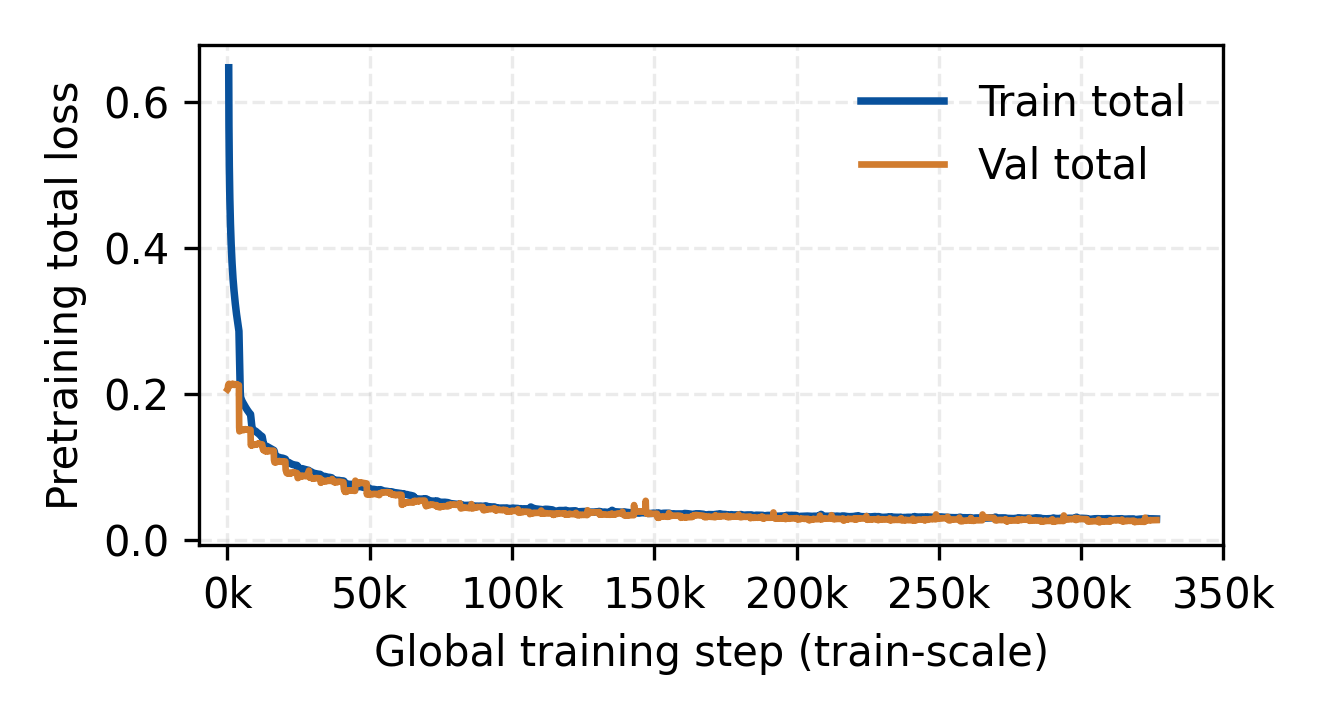
\includegraphics[width=\columnwidth]{figures/pretrain_loss_curve.png}
  \caption{\textbf{EnsembleEGNN pretraining loss dynamics.} Trajectories of the training loss (50-step moving average) and validation loss plotted against global training steps, illustrating stable model convergence on the CREMP dataset.}
  \label{fig:pretrain_loss}
\end{figure}

\subsection{Dataset and Protocol}
\label{sec:dataset}

For quantitative evaluation, we used CREMP-CycPeptMPDB~\cite{grambow2024cremp}, which contains cyclic peptide conformers paired with artificial membrane permeation scores, yielding $n=3003$ labeled measurements before boundary filtering. We removed exact boundary targets at $\log(P_{\text{app}})$=-10.0, -8.0, and -4.0, resulting in a final evaluation set of $n=2979$. We ran 5-fold cross-validation with fixed splits and report fold-wise and aggregate metrics over all held-out examples. In each run, 3 folds were used for training, 1 fold for validation, and 1 fold is kept as an unseen test fold used only for post-training prediction. EnsembleEGNN uses all-atom representations (i.e., atom-level node tokens and conformer coordinates) with 12 nearest neighbors, and BERT uses 1D sequence. The target is $\log(P_{\text{app}})$, and we evaluated MAE, RMSE, Pearson $r$, and $R^2$. All models used the same data splits and fine-tuning protocol (\autoref{tab:hyperparameters}). 

\subsection{Baselines}
\label{sec:baselines}

We compared four transfer variants under identical training and evaluation splits: (1) \textbf{BERT-only}, a sequence-only baseline utilizing the PeptideCLM-2- encoder \cite{feller2026scaling}; (2) \textbf{EnsembleEGNN-random-init}, the geometric model trained from random initialization without pretraining; (3) \textbf{EnsembleEGNN}, the pretrained geometric model; and (4) \textbf{Hybrid}, the full co-training EnsembleEGNN and PeptideCLM-2 with concatenated embeddings.

\subsection{Results}
\label{sec:results}

\begin{table*}[ht]
  \centering
  \caption{\textbf{Model performance metrics.} Cross validation of predictive accuracy on heldout CREMP-CycPeptMPDB data ($n=2979$). Values are reported as the mean $\pm$ standard error across 3 independent training replicates.}
  \label{tab:performance_metrics}
  \small
  \begin{tabular}{lcccc}
    \toprule
    \textbf{Model} & \bm{$R^2$} & \textbf{Pearson} \bm{$r$} & \textbf{MAE} & \textbf{RMSE} \\
    \midrule
    Random-init & 0.005 $\pm$ 0.004 & 0.113 $\pm$ 0.016 & 0.457 $\pm$ 0.003 & 0.601 $\pm$ 0.001 \\
    BERT-only & 0.439 $\pm$ 0.053 & 0.667 $\pm$ 0.035 & 0.334 $\pm$ 0.014 & 0.451 $\pm$ 0.022 \\
    EnsembleEGNN & 0.477 $\pm$ 0.009 & 0.699 $\pm$ 0.009 & 0.319 $\pm$ 0.002 & 0.436 $\pm$ 0.004 \\
    Hybrid & \textbf{0.538 $\pm$ 0.029} & \textbf{0.737 $\pm$ 0.016} & \textbf{0.304 $\pm$ 0.008} & \textbf{0.409 $\pm$ 0.013} \\
    \bottomrule
  \end{tabular}
\end{table*}

\begin{table}[ht]
  \centering
    \caption{\textbf{Detailed fold-wise \bm{$R^2$} evaluation.} Comparison of predictive performance across five distinct test folds. Results represent the mean $\pm$ standard error of three independent replicates, illustrating the relative stability of the BERT-only, EnsembleEGNN, and Hybrid architectures on different slices of the data.}
  \label{tab:conformer_count}
  \small
  \begin{tabular}{lccc}
    \toprule
    \textbf{Fold} & \textbf{BERT-only} & \textbf{EnsembleEGNN} & \textbf{Hybrid} \\
    \midrule
    1 & 0.426 $\pm$ 0.019 & 0.503 $\pm$ 0.007 & \textbf{0.565 $\pm$ 0.011} \\
    2 & 0.472 $\pm$ 0.026 & 0.456 $\pm$ 0.012 & \textbf{0.494 $\pm$ 0.035} \\
    3 & 0.430 $\pm$ 0.061 & 0.509 $\pm$ 0.031 & \textbf{0.553 $\pm$ 0.018} \\
    4 & 0.462 $\pm$ 0.057 & 0.451 $\pm$ 0.016 & \textbf{0.526 $\pm$ 0.054} \\
    5 & 0.402 $\pm$ 0.060 & 0.460 $\pm$ 0.012 & \textbf{0.552 $\pm$ 0.018} \\
    \bottomrule
  \end{tabular}
\end{table}

Overall performance on the PAMPA dataset details the necessity of the pretrained conformer-aware approach (Table~\ref{tab:performance_metrics}). While the randomly initialized EnsembleEGNN performed near random ($R^2$ = 0.005), pretraining the model on CREMP outperformed the sequence-only BERT baseline ($R^2$ = 0.477 vs. 0.439). The co-trained Hybrid model ultimately achieved the strongest aggregate metrics, improving the final $R^2$ to 0.538, resulting in a Pearson $r$ of 0.737.

\begin{figure}[ht]
  \centering
  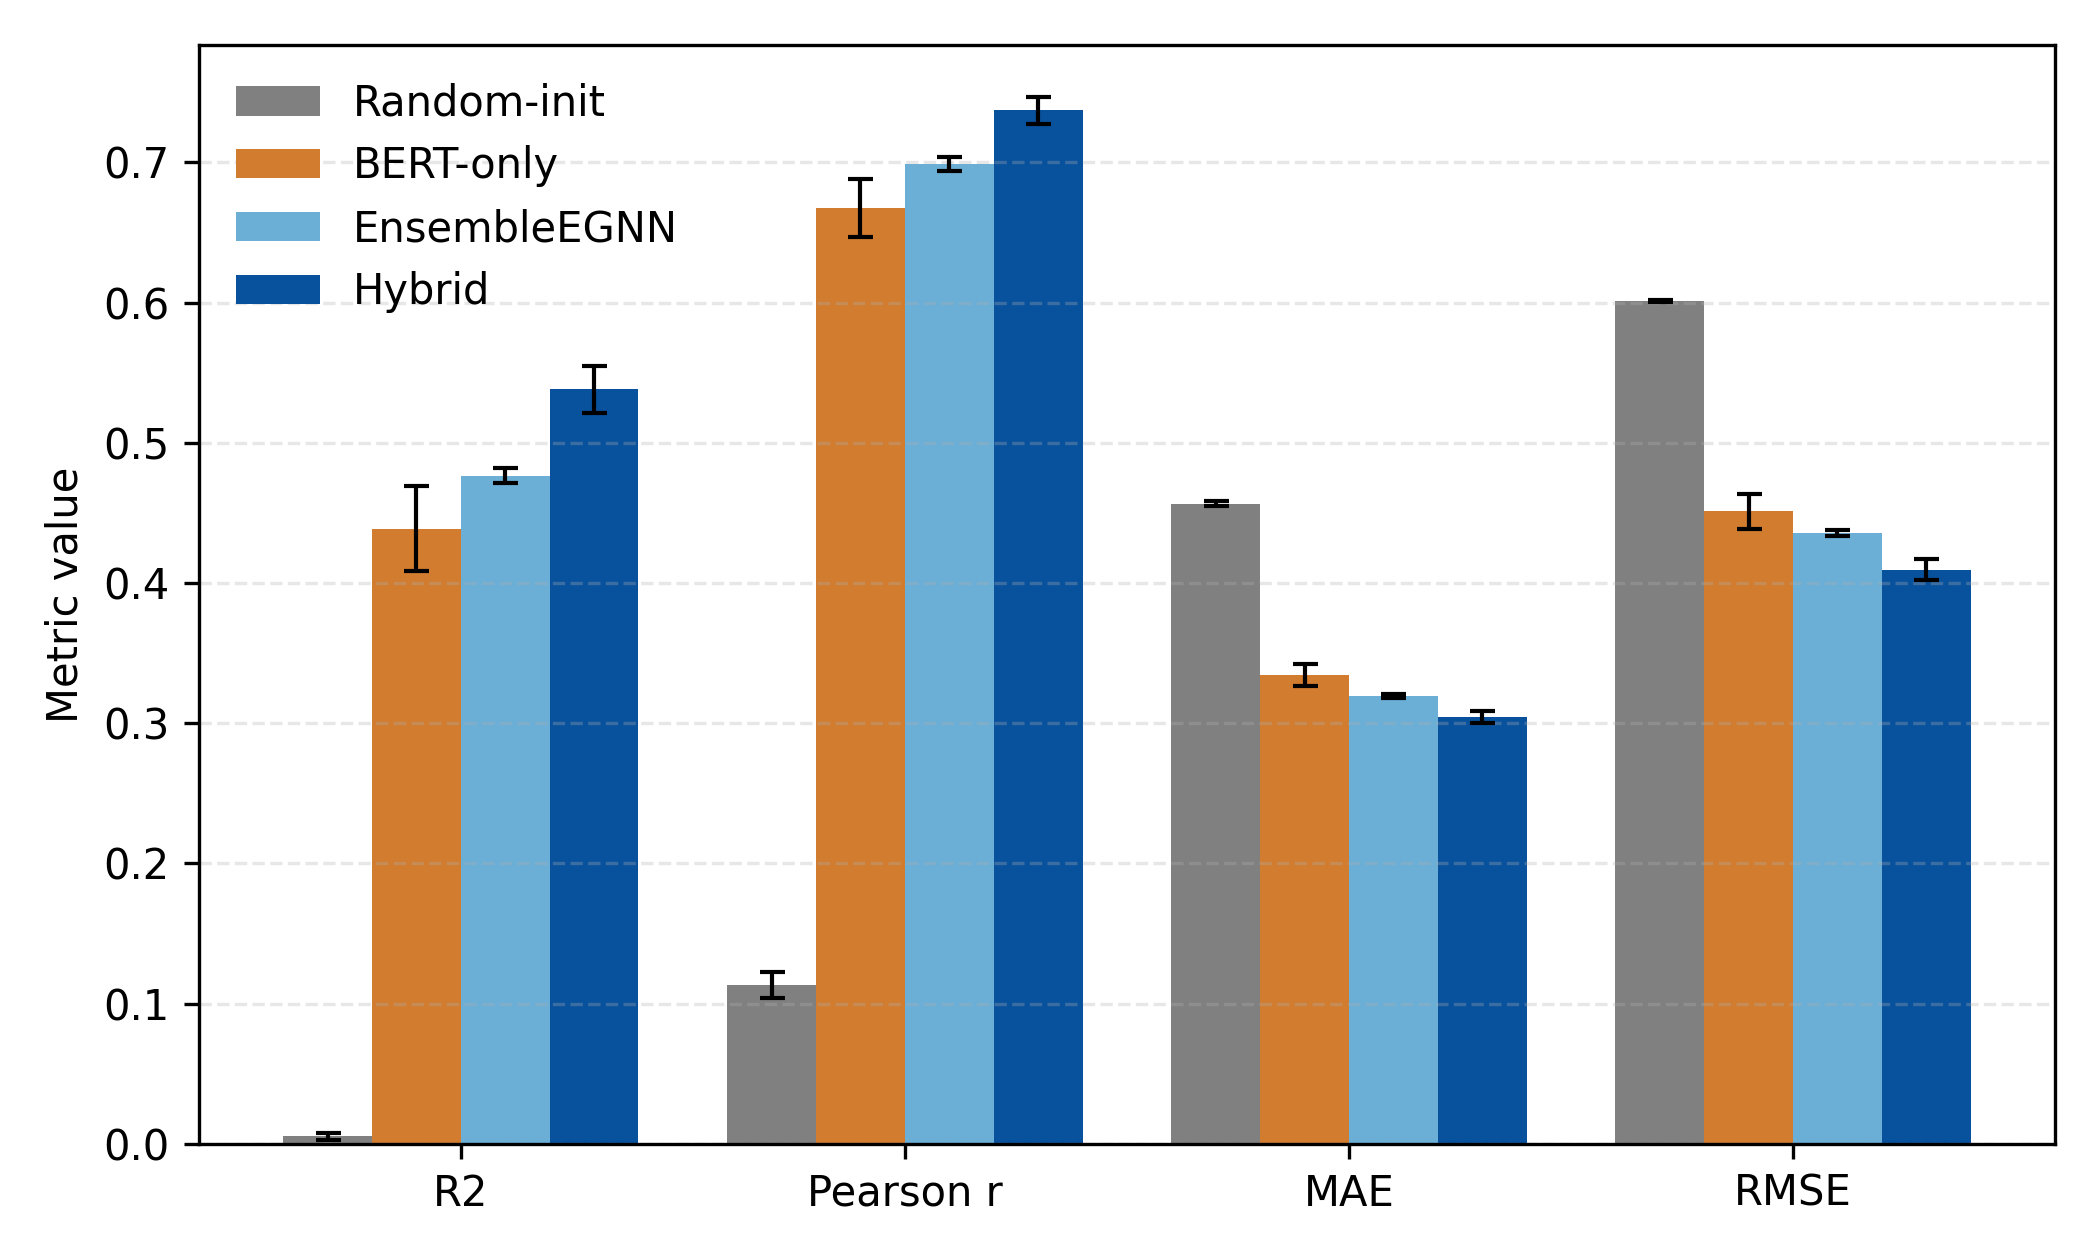
\includegraphics[width=\columnwidth]{figures/cv_overall_metrics.png}
  \caption{\textbf{Aggregate performance across cross-validation folds.} Comparison of mean evaluation metrics for the EnsembleEGNN w/o pretraining, BERT-only, EnsembleEGNN pretrained, and Hybrid architectures on the held-out PAMPA dataset. The co-trained Hybrid model consistently achieves the strongest overall performance across all evaluated metrics. Error bars represent the standard error across three independent training runs.}
  \label{fig:overall_metrics}
\end{figure}

The Hybrid model consistently achieved the strongest mean $R^2$ performance across all 5 individual cross-validation folds (Table~\ref{tab:conformer_count}). Visualizations of the overall metrics further demonstrate this performance gap (Fig.~\ref{fig:overall_metrics}), supported by per-model held-out prediction scatter plots (Fig.~\ref{fig:parity}). Notably, the EnsembleEGNN model requires pretraining in order to achieve performance above random for 20 epoch finetuning.

\begin{figure}[tb]
  \centering
  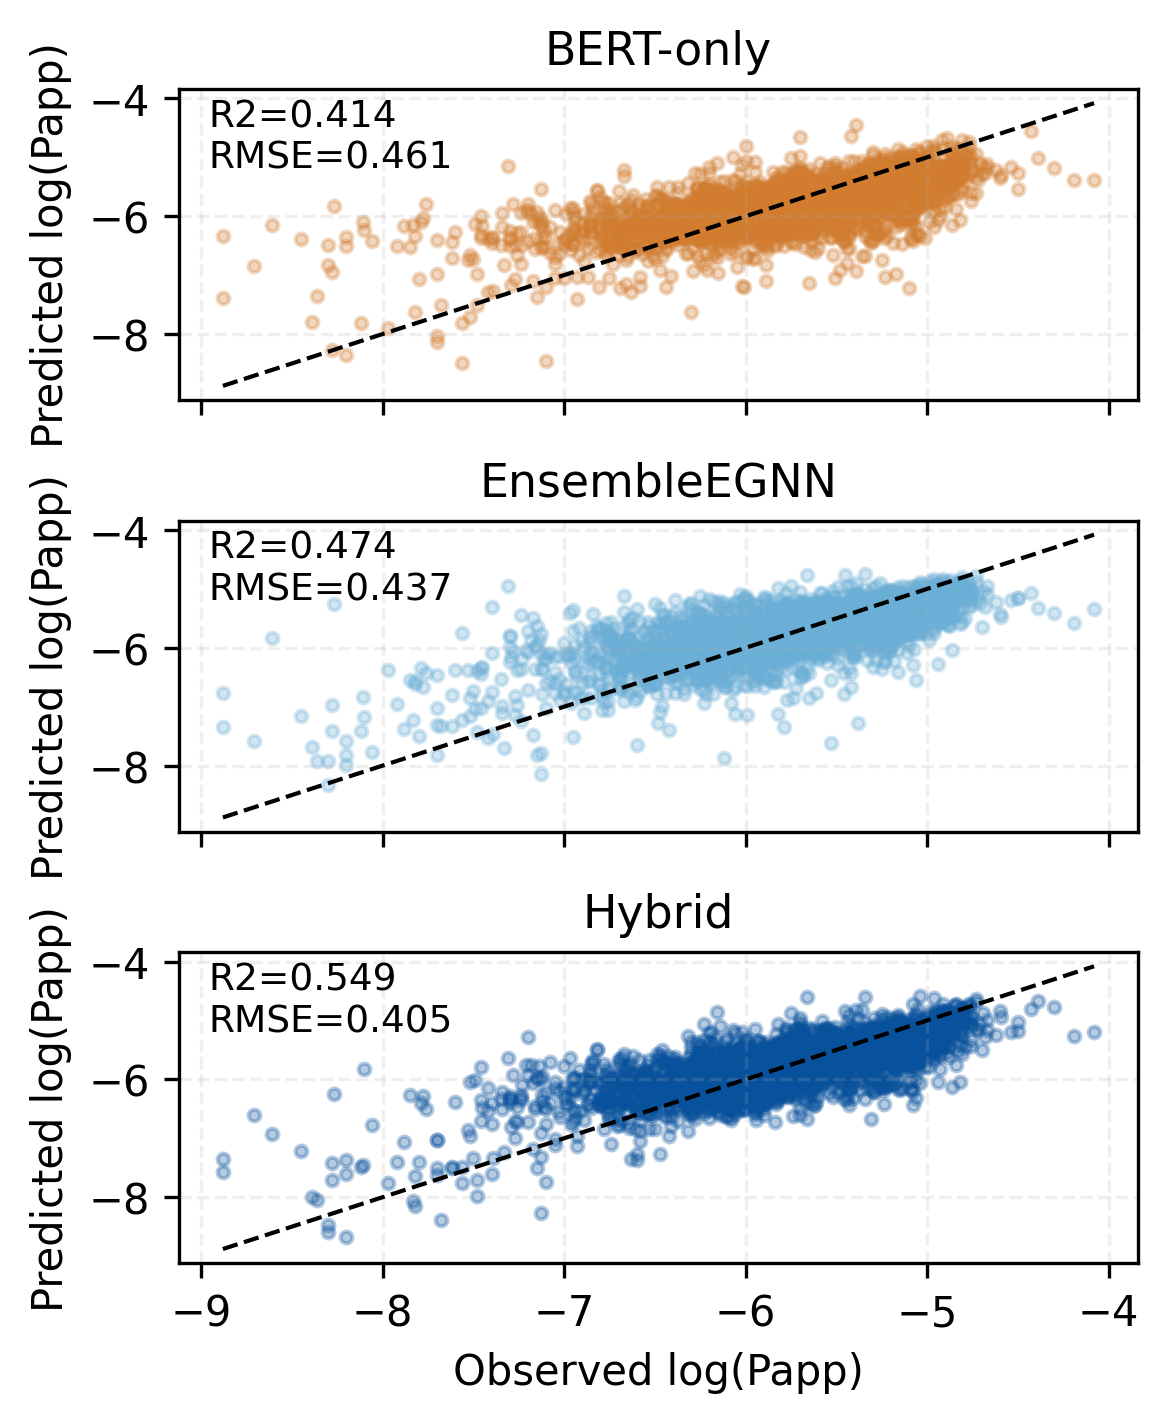
\includegraphics[width=\columnwidth]{figures/cv_parity.png}
  \caption{\textbf{Predictive performance on held-out PAMPA measurements.} Parity plot comparing predicted versus experimental $\log(P_{\text{app}})$ values across the complete evaluation set ($n=2979$). Proximity to the diagonal identity line illustrates the prediction accuracy, highlighting the tighter correlation achieved by the Hybrid model.}
  \label{fig:parity}
\end{figure}


% ============================================================
\section{Discussion}
\label{sec:discussion}
% ============================================================

\paragraph{Ensemble representations as a GFM primitive.}
The conformer aggregation problem is not unique to peptides. Protein loop flexibility~\citep{marks2018predicting}, RNA secondary-structure ensembles~\citep{bauskar2025boltzmann}, and small-molecule tautomers~\citep{greenwood2010towards} all involve distributions over molecular structures. Our results suggest that explicitly learning from multiple conformers, rather than collapsing to a single structure upfront, can be a useful design principle for molecular foundation models.

\paragraph{Transfer learning and scalability.}
Attempting to train the geometric conformer model from random initialization on the downstream task failed entirely ($R^2 = 0.005$). The shared EGNN backbone must be pretrained on CREMP with self-supervised objectives to establish meaningful physical priors before transferring to downstream regression tasks. This gives hope that with expanded study, the model may be able to generalize outside the training distribution, as has been shown with transfer learning from a model pretrained on a larger corpus. Consistent with the foundation model paradigm, we anticipate that by scaling both conformer datasets and model capacity, the representation advantages of self-supervised geometric pretraining will compound. Notably, the current architecture at 11.3M parameters outperforms a BERT-style architecture that contains 114M parameters.

\paragraph{Computational efficiency and scalability.}
Utilizing a SAB with inducing points makes conformer fusion effectively linear in the number of conformers when the number of inducing points is fixed, rather than quadratic as in standard self-attention. Should future applications require modeling larger conformer sets, this separation between per-conformer geometric encoding and ensemble pooling should remain useful. The same decomposition also allows the model to scale independently with molecule size and with the number of conformers.

\paragraph{Limitations and future work.}
Our approach has three primary limitations. Architecturally, the current EGNN layers perform message passing only within each conformer; interactions across conformers are introduced later through conformer pooling rather than through explicit cross-conformer message passing. Data-wise, this study was strictly bounded by the coverage and accuracy of the precomputed CREMP ensembles. Finally, while our hybrid model outperforms the sequence baseline on this benchmark, the CREMP-CycPeptMPDB dataset remains a low-data regime ($n=2979$), which warrants caution when making generalized cross-paper comparisons. Future work will explore richer cross-conformer interaction mechanisms and integrate scalable, high-fidelity conformer generation to expand beyond existing library constraints.

% ============================================================
\section{Conclusion}
\label{sec:conclusion}
% ============================================================
We present EnsembleEGNN, an ensemble geometric foundation model that encodes each conformer with shared EGNN layers and pools those conformer representations into a single thermodynamically informed embedding. Through multi-task self-supervised pretraining on CREMP, the model learns to recover masked tokens, refine noisy coordinates, and preserve coarse ensemble geometry. With transfer learning to the CREMP-CycPeptMPDB benchmark ($n=2979$), EnsembleEGNN outperforms a pretrained BERT architecture. The hybrid transfer model further improves over the sequence-only baseline by $+0.099$ in $R^2$ and $+0.070$ in Pearson $r$, with correspondingly lower MAE and RMSE. More broadly, this work shows that directly learning from conformer ensembles can improve cyclic-peptide representation learning.

% ============================================================
\clearpage
\section*{Impact}

This paper presents work whose goal is to advance the field of machine learning for molecular design and early stage drug discovery. By improving property prediction for highly flexible cyclic peptides, architectures like EnsembleEGNN can help accelerate the development of novel therapeutics and reduce the time and resource costs associated with high throughput physical screening. While advancing computational drug design has overwhelmingly positive societal benefits, we acknowledge that machine learning models in this domain should not be utilized in isolation. Predictions generated by our foundation model are intended to serve as hypothesis generating tools to guide wet lab validation, rather than definitive claims of biological efficacy or safety. We do not foresee any direct negative ethical consequences arising specifically from the methodological advancements presented in this work.

\section*{LLM usage}
LLMs were used during the preparation of the manuscript solely as writing aids to catch typographical and grammatical errors and to improve writing style and latex formatting.

\section*{Code availability}
Removed for double-blind review.

\section*{Acknowledgments}
% ============================================================

Anonymized for double-blind review.
% ============================================================
\bibliography{references}
\bibliographystyle{icml2026}
% ============================================================

\clearpage
\setcounter{table}{0}
\renewcommand{\thetable}{S\arabic{table}}


\begin{table*}[ht]
\section*{Supplemental Table}
\vspace{0.3cm}
  \centering
  \caption{\textbf{EnsembleEGNN architecture and training hyperparameters.} Summary of the verified backbone, conformer-fusion, pretraining, and downstream optimization settings used in the reported experiments. Values reflect the effective configuration of the reported all-atom EnsembleEGNN runs.}
  \label{tab:hyperparameters}
  \small
  \resizebox{2\columnwidth}{!}{%
  \begin{tabular}{llc}
    \toprule
    \textbf{Category} & \textbf{Parameter} & \textbf{Value} \\
    \midrule
    \textbf{EGNN backbone} & Parameters & 7.85M \\
    & Number of EGNN layers ($L$) & 6 \\
    & Effective hidden dimension ($d$) & 448 \\
    & Number of neighbors ($k$) & 12 \\
    & Dropout & 0.1 \\
    \midrule
    \textbf{Conformer fusion} & Parameters & 3.42M \\
    & Fusion mode & \texttt{setattn} \\
    & Set-attention blocks & 2 \\
    & Inducing points & 4 \\
    & Attention heads & 8 \\
    & Conformer-prior bias & enabled \\
    \midrule
    \textbf{Pretraining: EnsembleEGNN} & Epochs & 80 \\
    & Batch size & 8 \\
    & Learning rate & $2 \times 10^{-4}$ \\
    & Weight decay & $1 \times 10^{-4}$ \\
    & Masking ratio & 15\% \\
    & Corruption probabilities (mask/random/keep) & 0.8 / 0.1 / 0.1 \\
    & Coordinate noise std ($\sigma$) & 0.15~\AA \\
    & Loss weights ($\lambda_{\mathrm{tok}}$, $\lambda_{\mathrm{coord}}$, $\lambda_{\mathrm{dist}}$) & 0.3 / 0.5 / 0.2 \\
    \midrule
    \textbf{Fine-tuning: EnsembleEGNN} & Epochs & 20 \\
    & Batch size & 8 \\
    & Learning rate & $1 \times 10^{-4}$ \\
    & Weight decay & $1 \times 10^{-4}$ \\
    & Regression head layers & 2 \\
    & Head dropout & 0.1 \\
    & Early stopping patience & 3 \\
    \midrule
    \textbf{Fine-tuning: BERT} & Encoder & \texttt{aaronfeller/peptideclm-2-hybrid-base} \\
    & Epochs & 20 \\
    & Batch size & 16 \\
    & Learning rate & $3 \times 10^{-4}$ \\
    & Weight decay & $1 \times 10^{-2}$ \\
    & Regression head layers & 2 \\
    & Head dropout & 0.1 \\
    & Early stopping patience & 3 \\
    \midrule
    \textbf{Fine-tuning: Hybrid} & Geometric init checkpoint & \texttt{best\_pretrain.pt} \\
    & Epochs & 20 \\
    & Batch size & 8 \\
    & Learning rates (head / ensemble / CLM) & $2 \times 10^{-4}$ / $1 \times 10^{-4}$ / $2 \times 10^{-5}$ \\
    & Weight decay & $1 \times 10^{-4}$ \\
    & Regression head layers & 2 \\
    & Head dropout & 0.1 \\
    & Early stopping patience & 3 \\
    \bottomrule
  \end{tabular}
  }
\end{table*}

\end{document}